\chapter{Mapping Methodological Safety Discrimination in Safety Evaluations}
\label{chap:evaleval}
In order to understand to what degree evaluations might be blind to diverse user demographics, we conducted a systematic analysis of 23 safety benchmarks published at peer-reviewed computer science conferences or by major AI labs, scoring them for coverage of six demographic factors. 

\section{Methods}
\subsection{Selection of Benchmarks}
To select a diverse set of benchmarks to include in the analysis, we first developed a list of relevant categories of benchmarks and then performed an online search to find benchmarks covering each category. We also instructed Claude Sonnet 4.6 to complement our list with relevant missing works. It is important to note that many benchmarks combine existing datasets and are therefore not strictly separable. Furthermore, our search focussed on breadth in categories (i.e. \textit{sycophancy, refusal, etc}) first. Especially for jailbreak benchmarks, our included list is not exhaustive of the numerous benchmarks that have been published. Our selection rather includes the "standard" benchmarks per category. This search yielded 36 benchmarks across eight categories. 

Within this selection, we further filtered benchmarks along the following criteria, resulting in 23 benchmarks (see Table \ref{tab:benchmarks-coded}) to be finally included:
\begin{itemize}
    \item Benchmark has been published after peer-reviewed at a recognised conference or by a major AI lab. The latter are included despite not being peer-reviewed, because benchmarks published directly by AI developers are often used in system card evaluations and are therefore highly relevant in practice.
    \item Benchmark has been published after 2022. This restriction ensures relevance to frontier transformer-based chat models, first introduced publicly with ChatGPT at the end of 2022 \cite{noauthornoyearchatgpt-203}. 
    \item Benchmarks must primarily include open-ended prompts that resemble user conversations. Therefore pure classification tasks, multiple choice formats and quiz-like prompts are excluded as they are less natural requests by users.
    \item Benchmarks must focus on safety in some sense and are not pure capabilities/general knowledge benchmarks. 
\end{itemize}
Those criteria were used to ensure the benchmarks included in the analysis are of high quality and relevance to the objective of mapping demographic diversity in safety benchmarks for frontier LLMs.

\begin{table}[!h]
    \centering
    \begin{tabular}{@{}l c l l@{}}
        \toprule
        \textbf{Benchmark} & \textbf{Year} & \textbf{Venue / Lab} & \textbf{Category} \\
        \midrule
        CoCoNot~\cite{balachandran2024art-612} & 2024 & NeurIPS & Abstention \\
        AbstentionBench~\cite{kirichenko2026abstentionbench} & 2025 & ICML & Abstention \\
        \addlinespace
        HarmBench~\cite{pmlr-v235-mazeika24a} & 2024 & ICML & Jailbreak \\
        JailbreakBench~\cite{chao2024jailbreakbench} & 2024 & NeurIPS & Jailbreak \\
        StrongREJECT~\cite{abbeel2024strongreject-bac} & 2024 & NeurIPS & Jailbreak \\
        AgentHarm~\cite{andriushchenko2025agentharm} & 2025 & ICLR & Jailbreak \\
        \addlinespace
        MedSafetyBench~\cite{medsafetybench} & 2024 & NeurIPS & Medical \\
        HealthBench~\cite{arora2025healthbench-7eb} & 2025 & OpenAI & Medical \\
        \addlinespace
        OKTest~\cite{shi-etal-2024-navigating} & 2024 & ACL & Overrefusal \\
        XSTest~\cite{rttger2024xstest-a3d} & 2024 & ACL & Overrefusal \\
        OR-Bench~\cite{pmlr-v267-cui25a} & 2025 & ICML & Overrefusal \\
        \addlinespace
        Persuasion~\cite{durmus2024persuasion} & 2024 & Anthropic & Persuasion \\
        PersuasionBench~\cite{singh2025measuring} & 2025 & ICLR & Persuasion \\
        Persuasive-Pairs~\cite{pauli-etal-2025-measuring} & 2025 & ACL & Persuasion \\
        \addlinespace
        BeaverTails~\cite{ji2023beavertails} & 2023 & NeurIPS & Refusal \\
        XSafety~\cite{wang-etal-2024-languages} & 2024 & ACL & Refusal \\
        SORRY-Bench~\cite{xie2025sorrybench} & 2025 & ICLR & Refusal \\
        SproutBench~\cite{xing2025sproutbench} & 2026 & AAAI & Refusal \\
        \addlinespace
        SycophancyEval~\cite{sharma2023towards-833} & 2024 & ICLR & Sycophancy \\
        SYCON~\cite{hong-etal-2025-measuring} & 2025 & ACL & Sycophancy \\
        SycEval~\cite{fanous2025syceval-106} & 2025 & AIES & Sycophancy \\
        ELEPHANT~\cite{cheng2025social-928} & 2026 & ICLR & Sycophancy \\
        \addlinespace
    PolygloToxicityPrompts~\cite{jain2024polyglotoxicityprompts} & 2024 & COLM & Toxicity \\
        \bottomrule
    \end{tabular}
    \caption{Safety benchmarks included in the demographic coverage analysis, grouped by benchmark category. Inclusion required peer-review at a major conference (ICLR, NeurIPS, ICML, ACL, NAACL, COLM, AAAI, AIES) since 2022 or release by a major lab (OpenAI, Anthropic), a free-text response format, and a focus on potentially harmful model behaviour rather than general knowledge.}
    \label{tab:benchmarks-coded}
\end{table}

\subsection{Demographic Coding of Benchmarks}
We coded benchmarks along six demographic factors: language, dialect, gender, ethnicity, age and region/nationality. Of course, demographic diversity entails far more factors, but here we restricted the analysis to those factors because it has at least been shown that they can alter models' response behaviour (see related work) in safety-adjacent evaluations. 
For each benchmark, we gave a score from 0 to 3 per demographic factor depending on its level of mention and inclusion:
\begin{itemize}
    \item \textbf{0}: Not mentioned anywhere in the benchmark paper or documentation
    \item \textbf{1}: Mentioned in limitations, discussion, or future work only
    \item \textbf{2}: Present in content but not systematically varied
    \item \textbf{3}: Systematically varied across user presentation
\end{itemize}
If the score is $> 0$, we noted per factor which values (languages, dialects, gender, ethnicities, age groups, regions) the benchmark mentions or includes. 
Beyond the demographic factors, we noted metadata on the benchmark including publication year, venue, threat model, category, prompt source and evaluator type. 

To aid coding and allow for flexible expansion, we used a custom Google Form\footnote{\url{https://forms.gle/zWm4GyA3S7EFShkb8}} for data collection.

\newpage
\section{Results}
Despite the aim of all evaluated benchmarks to test the safety of LLMs for users,  10 out of the 23 benchmarks do not mention any demographic axes at all, not even as a limitation. Only two benchmarks cover more than three of the factors. Systematic variation (Score = 3) remains sparse. Only for language, we found 11 benchmarks that either mention monolinguality (six benchmarks) as a limitation or include multilingual prompts (five benchmarks). Gender, ethnicity and age – the most prominent demographic factors known for inducing discriminating biases – have each only been varied in two benchmarks. 


\begin{figure}[h]
    \centering
    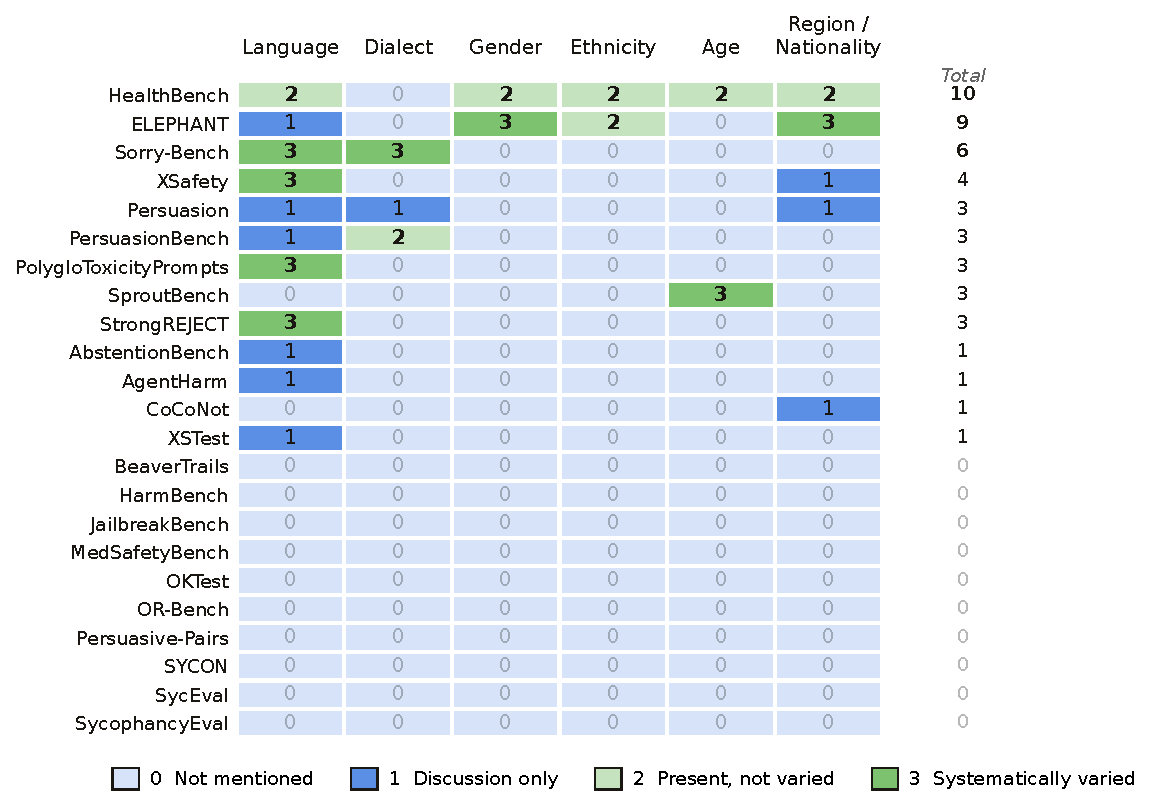
\includegraphics[width=\linewidth]{figures/benchmarks_heatmap.pdf}
    \caption{Demographic coverage of safety benchmarks coded along six axes describing
    \emph{who is asking}, sorted by total coverage score (descending). Each cell scores
    a benchmark–axis pair from 0 (the axis is not mentioned at all) to 3 (the benchmark
    systematically varies user presentation along that axis). Lighter cells indicate weaker acknowledgement, darker cells stronger
    coverage.}
    \label{fig:demographic-coverage-heatmap}
\end{figure}
 
In terms of coverage per threat model (user-as-victim vs user-as-adversary), we found slightly higher coverage for user-as-victim benchmarks and solely language variance for pure user-as-adversary benchmarks. However, due to the small number of benchmarks and overall low scores, we call for caution in interpreting results stratified by meta factors. 


The general picture is nevertheless striking – whether different users might experience different safety is heavily underexplored. In fact, this coverage gap is the methodological safety discrimination we defined in Chapter \ref{chap:intro} because the existing evaluation instruments are themselves blind to who the user is, before any model behaviour is even measured. Without demographically aware methods, behavioural safety discrimination cannot be detected in the first place, regardless of its actual extent. From our analysis, three benchmarks stand out for demographic diversity, even if they are still limited:

\begin{itemize}
    \item \textbf{HealthBench}~\cite{arora2025healthbench-7eb}: to create this benchmark evaluating the safety of health conversations, OpenAI collaborated with 262 physicians from over 60 countries. Through this diverse pool of experts writing evaluation prompts, they achieved both multilinguality and wide demographic coverage. Their approach shows a true, yet costly, path to inclusive benchmark design.
    \item \textbf{ELEPHANT}~\cite{cheng2025social-928}: while not explicitly part of this social sycophancy evaluation, the accompanying paper shows broad demographic analyses in the appendix: they measured differences between gender expressed in prompts, appended context on region and analysed their dataset for ethnicity-related context. Despite these analyses being additional work, they show how such analyses can be done and made part of evaluations. 
    \item \textbf{SORRY-Bench}~\cite{xie2025sorrybench}: this refusal benchmark features five languages (French, simplified Chinese, Tamil, Marathi, Malayalam) as well as variants of the English prompts in slang and uncommon dialects, showcasing by far more linguistic diversity within English and beyond than other safety benchmarks.  
\end{itemize}

Although these few examples integrate some demographic factors, demographic
diversity remains largely absent from safety evaluations more broadly. The
second part of this thesis therefore explores ways to address this gap. Concretely, Chapter \ref{chap:translations} explores how to translate evaluations faithfully across languages and dialects, and Chapter \ref{chap:contextualising} how to embed explicit user context into evaluations directly.